\documentclass[11pt]{article}

\usepackage[margin=1in]{geometry}
\usepackage[T1]{fontenc}
\usepackage[utf8]{inputenc}
\usepackage{lmodern}
\usepackage{graphicx}
\usepackage{booktabs}
\usepackage{array}
\usepackage{hyperref}
\usepackage{xcolor}

\hypersetup{
  colorlinks=true,
  linkcolor=blue!55!black,
  citecolor=blue!55!black,
  urlcolor=blue!55!black
}

\title{Reading Scene Text for Visual Question Answering}
\author{Chris Chen \and Charles Wang}
\date{Spring 2026}

\begin{document}
\maketitle

\section{Introduction}

Many visual question answering systems can describe objects, scenes, and simple spatial relations, but they still fail when the answer depends on text inside the image. Text is common in real visual environments: product labels, street signs, receipts, medical device screens, drug packaging, forms, dashboards, and instructions often carry the information needed to answer a question. A model that ignores or misreads this text may produce an answer that is fluent but wrong.

This project studies that failure mode using TextVQA, a benchmark whose questions require reading and reasoning over scene text \cite{singh2019textvqa}. Each example pairs an image with a natural-language question and multiple human answers. The model must identify which visible text is relevant, read it correctly, and return a concise answer that matches the annotators' responses. We use the predefined TextVQA train and validation splits from Hugging Face, with 34.6k training examples and 5k validation examples.

This capability is relevant to medicine and health-adjacent workflows because visual information is often mixed with text: medication labels, monitor readouts, intake forms, appointment slips, nutrition labels, and device instructions. This project does not train on protected clinical data, but TextVQA provides a controlled benchmark for a related capability: answering questions from images where written text carries the key evidence.

Our goal is to measure how well a modern open-source vision-language model handles this text-centric setting and then improve it with a reproducible adaptation method. We use Qwen2.5-VL-3B-Instruct as the base model because it is small enough for accessible multi-GPU fine-tuning while still being designed for document, chart, and text-rich visual understanding \cite{bai2025qwen25vl}. The main improvement method is LoRA fine-tuning, which freezes the pretrained model weights and trains low-rank adapter matrices in selected transformer modules \cite{hu2022lora}. The experiments compare zero-shot inference, LoRA fine-tuning, prompt-based OCR instructions, LoRA target-module choices, and image-resolution changes under the same validation split and scoring code.

\section{Background}

\subsection{Text-Centric Visual Question Answering}

TextVQA was introduced to evaluate VQA models on scene text reading, a capability beyond standard visual object recognition \cite{singh2019textvqa}. The original work showed that standard VQA systems struggled on questions grounded in text and proposed Look, Read, Reason, and Answer (LoRRA), a model that combines visual features, OCR tokens, and question context. The benchmark remains useful for modern VLMs because the hard cases extend beyond OCR. The model must also decide which text matters, normalize short answers, and avoid hallucinating plausible but unseen words.

Evaluation follows the VQA-style multi-answer setup. Each prediction is compared against the set of human answers, and TextVQA soft accuracy gives partial credit based on annotator agreement. This is more appropriate than a single exact-match label because valid answers can vary in spelling, punctuation, and specificity. In this report, TextVQA soft accuracy is the primary metric, while exact match, token F1, BLEU, METEOR, and ROUGE-L provide secondary views of answer quality.

\subsection{Modern Vision-Language Models}

Recent VLMs differ in how they connect images to language models. BLIP-2 uses a frozen image encoder, a frozen language model, and a trainable Q-Former bridge to reduce the cost of vision-language pretraining \cite{li2023blip2}. LLaVA connects a vision encoder to a language model and improves instruction-following behavior through visual instruction tuning \cite{liu2023llava}. These designs helped move VLMs from task-specific architectures toward general-purpose visual assistants, but text-heavy images still stress their visual resolution, OCR alignment, and answer normalization.

Qwen2.5-VL is a more recent open-source VLM family with explicit emphasis on visual recognition, document parsing, localization, and dynamic-resolution processing \cite{bai2025qwen25vl}. Those properties make Qwen2.5-VL-3B-Instruct a strong fit for TextVQA: the model is compact enough for our compute budget, supports instruction-style prompting, and is built for the kinds of text-rich visual inputs that dominate this benchmark.

\subsection{Parameter-Efficient Fine-Tuning}

Full fine-tuning updates all model weights and can be costly for large VLMs. LoRA instead freezes the pretrained weights and inserts low-rank trainable matrices into selected linear layers \cite{hu2022lora}. This reduces memory use and checkpoint size while allowing the model to adapt to a downstream task. In this project, the vision side remains frozen, and LoRA adapters are applied to language-model attention and MLP projection modules. This choice matches the goal of improving answer generation and text-conditioned reasoning without retraining the whole multimodal backbone.

\section{Methodology}

\subsection{Data Pipeline}

The data pipeline downloads TextVQA from the Hugging Face dataset \texttt{lmms-lab/textvqa} and preprocesses the train and validation splits into local JSONL files. Each raw row is normalized into a common schema containing the question id, image id, question text, answer list, majority target answer, OCR tokens, and cached image path used during inference. Images are converted to RGB JPEGs and resized with a longest side of 448 pixels for the main runs. 
For training, each example is converted into a Qwen chat-style multimodal sequence. The user message contains the image and the prompt: ``Question: \{question\}. Answer with the shortest correct text from the image.'' The assistant message contains the majority human answer from the TextVQA answer list. This keeps the supervised target concise and close to the benchmark answer format.

\subsection{Base Model and Input Formatting}

The main model is \texttt{Qwen/Qwen2.5-VL-3B-Instruct}. The model is loaded with bfloat16 weights, scaled dot-product attention, and Qwen's processor with the configured dynamic pixel range. For distributed inference, each process maps the model to its local GPU. For distributed training without 4-bit quantization, the model is loaded without an automatic device map so that \texttt{Accelerate} and the Hugging Face \texttt{Trainer} can manage the process-local model placement.

Both training and inference use Qwen's chat template and \texttt{qwen-vl-utils} to prepare image inputs. At inference time, the prompt template asks the model to answer only the question, and generation uses greedy decoding with a maximum of 32 new tokens. This decoding choice reduces variation across runs and matches the short-answer structure of TextVQA.

The codebase also includes \texttt{Salesforce/blip2-opt-2.7b} as a secondary model-comparison path. BLIP-2 is loaded with bfloat16 weights through the Hugging Face BLIP-2 generation API and processor. Its inference path uses a BLIP-2-specific prompt template and a cleanup step that removes echoed prompts or answer prefixes from OPT decoding outputs before scoring. This lets the experiments compare Qwen, a newer native multimodal instruction model, with BLIP-2, a frozen-vision/Q-Former/OPT bridge architecture.

\subsection{LoRA Fine-Tuning}

The improvement method is parameter-efficient LoRA fine-tuning. The vision side of the model is frozen, and LoRA adapters are inserted into the language-model attention and MLP projection layers: \texttt{q\_proj}, \texttt{k\_proj}, \texttt{v\_proj}, \texttt{o\_proj}, \texttt{gate\_proj}, \texttt{up\_proj}, and \texttt{down\_proj}. This design lets the model adapt its text-conditioned reasoning and answer generation while avoiding the cost of updating the full VLM.

For BLIP-2, the same training configuration is reused where possible. The full BLIP-2 LoRA configuration targets OPT attention and feed-forward modules together with Q-Former query/value projections, while the Q-Former-only ablation targets only the bridge projections. This isolates the comparison to architecture and adapter placement while holding the dataset, optimizer schedule, and validation protocol fixed.

\begin{center}
  \textbf{Table 1: Main LoRA training configuration.}\\[0.5em]
  \begin{tabular}{ll}
    \toprule
    Setting & Value \\
    \midrule
    Base model & Qwen2.5-VL-3B-Instruct \\
    Trainable method & LoRA adapters \\
    LoRA rank / alpha / dropout & 16 / 32 / 0.05 \\
    Frozen modules & Vision-side parameters \\
    Epochs & 2 \\
    Per-device batch size & 2 \\
    Gradient accumulation & 4 steps \\
    Effective batch size & 32 with 4 GPUs \\
    Learning rate & $1\times10^{-4}$ \\
    Scheduler / warmup & Cosine / 3\% warmup \\
    Precision & bfloat16 \\
    Max sequence length & 2048 tokens \\
    Seed & 42 \\
    \bottomrule
  \end{tabular}
\end{center}

Training uses the Hugging Face \texttt{Trainer} with gradient checkpointing enabled, tensorboard logging every 25 steps, checkpointing every 500 steps, and at most three saved checkpoints. A 512-example holdout is taken from the end of the training split for training-time evaluation, so the official validation split remains reserved for final model comparison. After training, the final LoRA adapter and processor are saved under \texttt{artifacts/checkpoints/lora-qwen25vl/best}.

\subsection{Evaluation Procedure}

All reported validation runs use the same processed TextVQA validation split of 5,000 examples. Prediction files are written as JSONL under \texttt{artifacts/predictions/}; each row preserves the question, answer list, image path, and model prediction. The same scoring entrypoint then computes metrics for zero-shot, fine-tuned, and ablation runs.

The primary metric is TextVQA soft accuracy. Before scoring, predictions and answers are lowercased, stripped of punctuation, and normalized by removing English articles. A prediction receives credit according to the number of matching human answers, capped at one: $\min(\mathrm{matches}/3, 1)$. Exact match and token-level F1 are included as additional answer-level metrics. BLEU, METEOR, ROUGE-1, ROUGE-2, and ROUGE-L provide secondary semantic-overlap measurements, and the evaluation code also supports an LLM-as-a-judge pass over a capped sample for qualitative similarity checking.

\subsection{Reproducibility}

The repository is organized around stage-specific scripts: download, preprocess, zero-shot inference, LoRA training, fine-tuned inference, ablations, and result generation. Each stage reads YAML configuration files from \texttt{configs/} and writes outputs under \texttt{artifacts/}. The main scripts are resume-friendly where possible, and generated metrics, plots, qualitative examples, and prediction files are kept separate from raw data and checkpoints. This structure makes the final numbers traceable to a specific model configuration, LoRA configuration, training configuration, and prediction file.

\section{Experimental Design}

\subsection{Splits and Controls}

The official TextVQA test labels are not included in the local artifacts, so all reported model comparisons use the predefined 5,000-example validation split. The training split is used only for LoRA adaptation. During training, 512 examples are held out from the end of the training split for training-time evaluation; this holdout is separate from the official validation split used for final reporting.

The experiments are designed to isolate one change at a time where possible. Within each architecture, the zero-shot and fine-tuned runs use the same validation examples, answer normalization, and greedy decoding setup. The Qwen LoRA target-module ablation changes only the adapter placement. The OCR-instruction and OCR-hint ablations change only the prompt and do not retrain the model. The high-resolution ablation changes the image preprocessing and model pixel budget while reusing the trained full-LoRA Qwen adapter. The BLIP-2 runs use the same split and scoring code, but they use BLIP-2's processor, prompt format, and architecture-specific LoRA targets.

\newpage
\subsection{Runs}

\begin{center}
\small
\textbf{Table 2: Validation runs used in the experimental comparison.}\\[0.5em]
\begin{tabular}{>{\raggedright\arraybackslash}p{0.21\linewidth}>{\raggedright\arraybackslash}p{0.25\linewidth}>{\raggedright\arraybackslash}p{0.40\linewidth}}
\toprule
Run & Purpose & Controlled comparison \\
\midrule
Qwen zero-shot & Baseline for Qwen's pretrained behavior on TextVQA. & No training; answer-only prompt; 448-pixel preprocessing; greedy decoding. \\
Qwen full LoRA & Main Qwen improvement method. & Same validation split and decoding as zero-shot; LoRA on attention and MLP projection modules. \\
Qwen attention-only LoRA & Tests whether MLP adapter targets matter. & Same training and evaluation setup as full LoRA, but adapters are limited to \texttt{q/k/v/o\_proj}. \\
Qwen OCR prompt & Tests prompt-only improvement without parameter updates. & Same pretrained model and validation split as zero-shot, but prompt explicitly asks the model to read visible text first. \\
Qwen OCR hint & Tests explicit OCR-token context. & Same pretrained model and validation split as zero-shot, but the prompt includes detected OCR tokens. \\
Qwen high-resolution & Tests whether text legibility is a bottleneck. & Same full-LoRA adapter, but validation images are preprocessed at 896 pixels and Qwen's max pixel budget is increased. \\
BLIP-2 zero-shot & Baseline for a Q-Former/OPT architecture. & No training; BLIP-2 prompt template; same validation split and metrics. \\
BLIP-2 full LoRA & Tests the same LoRA recipe on BLIP-2. & Same training hyperparameters as Qwen; adapters target OPT and Q-Former modules. \\
BLIP-2 Q-Former-only & Tests whether adapting only the bridge is sufficient. & Same BLIP-2 setup, but LoRA is limited to Q-Former query/value projections. \\
BLIP-2 OCR hint & Tests OCR-token prompting for BLIP-2. & Same BLIP-2 zero-shot model, but the prompt includes detected OCR tokens. \\
\bottomrule
\end{tabular}
\end{center}

These runs correspond to the prediction and metric files under \texttt{artifacts/predictions/} and \texttt{artifacts/metrics/}.

\subsection{Evaluation Metrics}

The primary metric is TextVQA soft accuracy on the validation split because it matches the multi-answer annotation protocol. Exact match and token F1 are reported to show answer-level agreement under the same normalization. BLEU, METEOR, ROUGE-1, ROUGE-2, and ROUGE-L are included as secondary semantic-overlap metrics, mainly to compare whether a method improves short answer quality beyond exact string agreement.

The final analysis also includes qualitative examples and an error taxonomy generated from the fine-tuned model predictions. This is necessary because aggregate accuracy cannot distinguish OCR failures, wrong-region selection, partial answers, empty outputs, and verbose or hallucinated answers. Those categories are used in the Results and Analysis section to explain where the model still fails after adaptation.

\section{Results and Analysis}

\subsection{Main Quantitative Results}

Table 3 reports validation metrics for all completed runs. Qwen2.5-VL is much stronger than BLIP-2 on this TextVQA setup: Qwen zero-shot reaches 0.6858 soft accuracy, while BLIP-2 zero-shot reaches 0.0603. Qwen LoRA fine-tuning improves soft accuracy to 0.7453, an absolute gain of 5.95 percentage points over the Qwen zero-shot baseline. The high-resolution Qwen evaluation gives the strongest result, reaching 0.8277 soft accuracy and 0.8881 token F1.

\begin{center}
\small
\textbf{Table 3: Validation performance on 5,000 TextVQA examples.}\\[0.5em]
\begin{tabular}{lrrrrr}
\toprule
Run & Soft acc. & Exact & Token F1 & BLEU & ROUGE-L \\
\midrule
Zero-shot Qwen & 0.6858 & 0.7262 & 0.7718 & 14.22 & 0.6155 \\
Full LoRA & 0.7453 & 0.7826 & 0.8104 & 46.64 & 0.6451 \\
Attention-only LoRA & 0.7192 & 0.7556 & 0.7879 & 44.07 & 0.6271 \\
OCR prompt & 0.6890 & 0.7280 & 0.7716 & 13.42 & 0.6175 \\
OCR hint & 0.7011 & 0.7378 & 0.7788 & 14.87 & 0.6210 \\
High-resolution & \textbf{0.8277} & \textbf{0.8668} & \textbf{0.8881} & \textbf{49.62} & \textbf{0.7021} \\
\midrule
BLIP-2 zero-shot & 0.0603 & 0.0680 & 0.1237 & 2.64 & 0.0942 \\
BLIP-2 LoRA & 0.0537 & 0.0578 & 0.1718 & 1.05 & 0.1219 \\
BLIP-2 Q-Former-only & 0.0582 & 0.0654 & 0.1187 & 0.12 & 0.0833 \\
BLIP-2 OCR hint & 0.0547 & 0.0606 & 0.1116 & 1.74 & 0.0882 \\
\bottomrule
\end{tabular}
\end{center}

\begin{center}
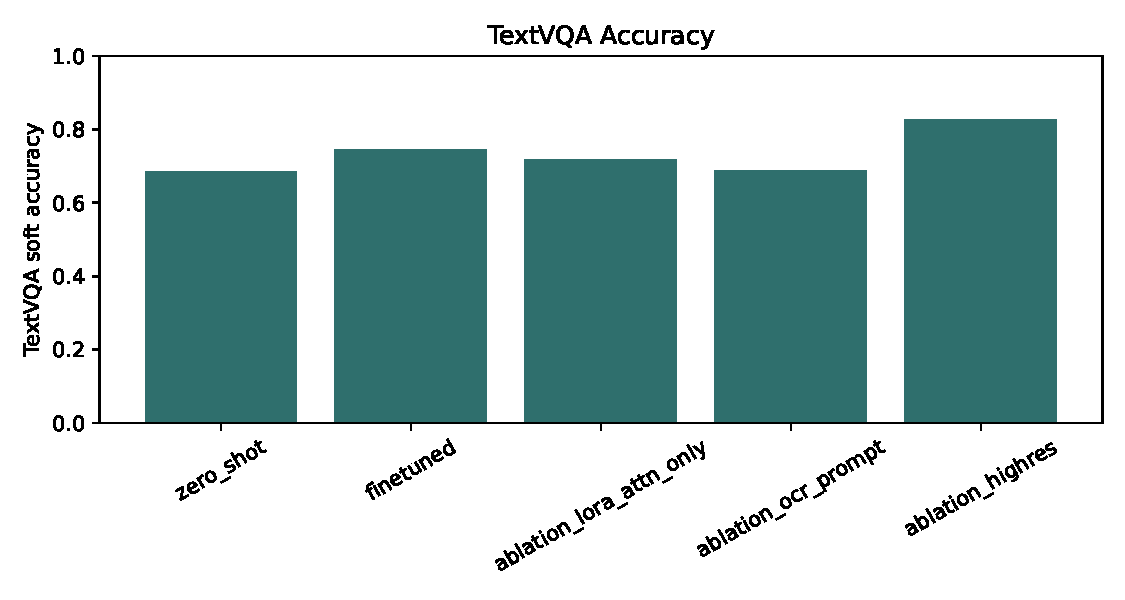
\includegraphics[width=\linewidth]{../artifacts/figures/accuracy_comparison.pdf}

\textbf{Figure 1:} TextVQA soft accuracy across the completed validation runs.
\end{center}

The main comparison shows that adaptation is useful for Qwen, but also that image legibility is a major limiting factor. Full LoRA improves over Qwen zero-shot while keeping the same 448-pixel preprocessing, which indicates that task-specific answer formatting and text-conditioned reasoning can be learned through lightweight adapters. The high-resolution run adds another 8.25 percentage points over the full-LoRA run, suggesting that many remaining Qwen errors are driven by insufficient visual detail, with language-side reasoning playing a smaller role. BLIP-2 performs far below Qwen in both zero-shot and LoRA settings, which suggests that this BLIP-2/OPT prompt-and-decoding setup is poorly matched to TextVQA's short OCR-heavy answers.

\subsection{Ablation Findings}

The Qwen ablations separate four design choices: adapter target modules, prompt-only OCR instruction, OCR-token context, and image resolution. Attention-only LoRA improves over zero-shot by 3.34 percentage points, but it remains 2.61 points below full LoRA. This supports the choice to adapt both attention and MLP projection layers. The OCR prompt changes the model instruction without changing weights and gives only a small gain over zero-shot, from 0.6858 to 0.6890. Adding OCR-token hints improves more, to 0.7011, but still remains far below LoRA fine-tuning and high-resolution evaluation.

The high-resolution ablation has the largest effect. It uses the trained full-LoRA adapter but preprocesses validation images at 896 pixels and raises Qwen's maximum pixel budget. Its accuracy gain is consistent with the task definition: many TextVQA answers are small numbers, brand names, or short printed phrases, so preserving more image detail directly improves the model's chance of reading the relevant text. The BLIP-2 ablations do not show the same pattern: full LoRA, Q-Former-only LoRA, and OCR-hint prompting all remain near 5-6\% soft accuracy. This points to a model-architecture or formatting mismatch at a level that hyperparameter tuning is unlikely to close.

\subsection{Question-Type Performance}

Figure 2 breaks down fine-tuned performance by the first word of the question. The model performs best on several closed-form categories such as ``does,'' ``is,'' and ``this,'' and performs worse on some open-ended categories such as ``when'' and ``what.'' This pattern is expected: questions asking for dates, prices, names, or arbitrary text strings require precise OCR and region selection, while yes/no or object-identification questions often have a smaller answer space.

\begin{center}
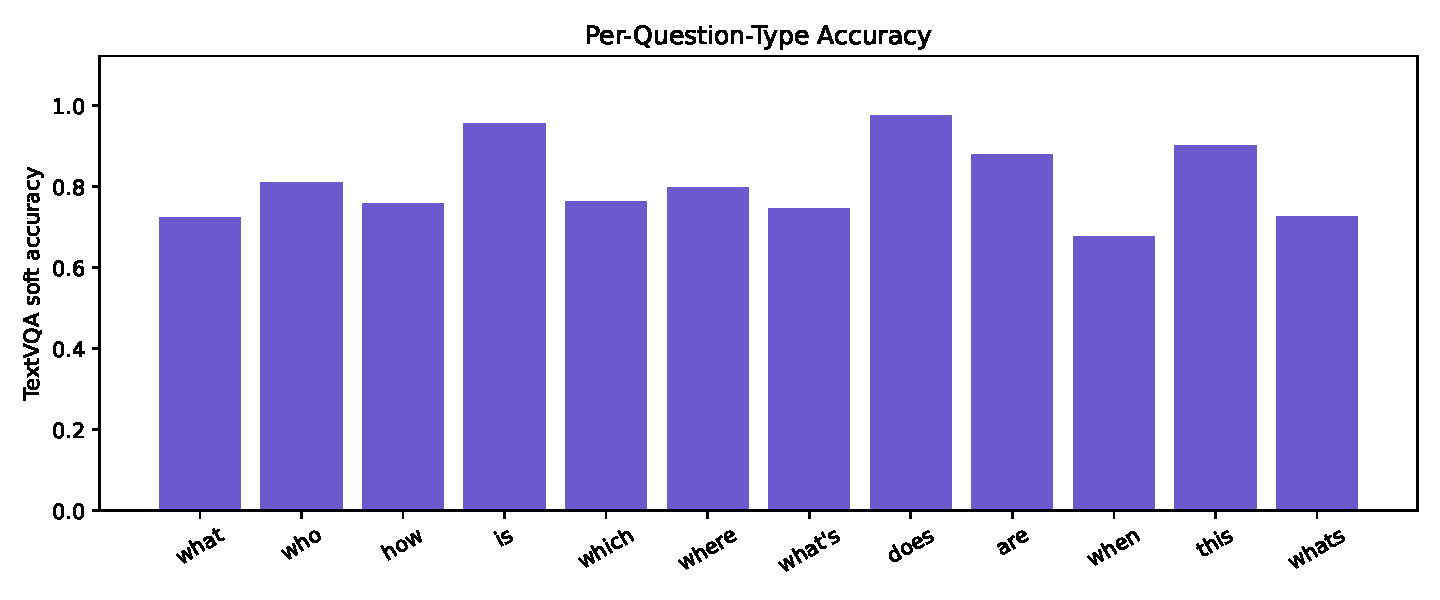
\includegraphics[width=0.90\linewidth]{../artifacts/figures/per_category_acc.pdf}

\textbf{Figure 2:} Fine-tuned TextVQA soft accuracy by question type.
\end{center}

\newpage
\subsection{Error Analysis}

The error taxonomy in Table 4 was generated from the full-LoRA validation predictions. The largest non-correct group is ``other,'' which contains heterogeneous failures that are not captured by the narrower rules. Among named failure modes, missed visible OCR is the dominant issue, accounting for 377 examples. Wrong text selection and partial matches are smaller but important because they show that the model often sees some relevant text but either chooses the wrong region or returns an incomplete answer.

\begin{center}
\small
\textbf{Table 4: Error taxonomy for the full-LoRA validation predictions.}\\[0.5em]
\begin{tabular}{lrr}
\toprule
Category & Count & Share \\
\midrule
Correct & 3913 & 78.26\% \\
Other & 537 & 10.74\% \\
Missed visible OCR & 377 & 7.54\% \\
Partial match & 113 & 2.26\% \\
Wrong text selected & 51 & 1.02\% \\
Empty answer & 6 & 0.12\% \\
Verbose or hallucinated & 3 & 0.06\% \\
\bottomrule
\end{tabular}
\end{center}

Qualitative examples support the same interpretation. The model correctly answers short text queries such as camera brands, city names, beer types, and ages when the relevant text is legible and well localized. Failures include reading a displayed time as ``10:08'' when the annotated answer is ``5:41,'' predicting a plausible watch brand when the answer set includes ``AP'' or ``unanswerable,'' and selecting the wrong name or product label in cluttered scenes. These examples show that the remaining errors go beyond answer formatting. They often require better OCR resolution, stronger grounding to the queried region, or explicit uncertainty when the text cannot be read.

\subsection{Sample Outputs}

Figure 3 shows the first two curated examples from \texttt{artifacts/sample\_outputs/}. The bottle example is a case where Qwen reads the relevant brand correctly across most variants, while BLIP-2 gives generic or wrong bottle names. The clock example shows a harder visual-detail failure: the annotated answer is 10:07, but every Qwen variant predicts a nearby wrong time, and BLIP-2 either returns no answer or a generic time.

\newpage
\begin{center}
\textbf{Figure 3: Representative sample outputs with source images and model predictions.}\\[0.75em]
\begin{minipage}[t]{0.47\linewidth}
\centering
\includegraphics[width=\linewidth]{../artifacts/sample_outputs/images/01_35514.jpg}\\[0.4em]
\scriptsize
\textbf{Question:} What is the brand of the second bottle from the left?\\
\textbf{Ground truth:} southern comfort\\[0.4em]
\setlength{\tabcolsep}{3pt}
\begin{tabular}{>{\raggedright\arraybackslash}p{0.34\linewidth}>{\raggedright\arraybackslash}p{0.54\linewidth}}
\toprule
Model & Prediction \\
\midrule
Qwen zero-shot & Southern Comfort \\
Qwen LoRA & southern comfort \\
Qwen OCR hint & Dewar's \\
Qwen high-res & southern comfort \\
BLIP-2 zero-shot & whiskey bottle \\
BLIP-2 LoRA & mccall's mark 70\% abv bourbon whiskey \\
BLIP-2 Q-Former & jack daniels whiskey \\
\bottomrule
\end{tabular}
\end{minipage}
\hfill
\begin{minipage}[t]{0.47\linewidth}
\centering
\includegraphics[width=\linewidth]{../artifacts/sample_outputs/images/02_34806.jpg}\\[0.4em]
\scriptsize
\textbf{Question:} What time does the top clock show?\\
\textbf{Ground truth:} 10:07\\[0.4em]
\setlength{\tabcolsep}{3pt}
\begin{tabular}{>{\raggedright\arraybackslash}p{0.34\linewidth}>{\raggedright\arraybackslash}p{0.54\linewidth}}
\toprule
Model & Prediction \\
\midrule
Qwen zero-shot & 10:25 \\
Qwen LoRA & 10:25 \\
Qwen attention-only & 10:35 \\
Qwen OCR hint & 10:10 \\
Qwen high-res & 10:25 \\
BLIP-2 zero-shot & empty \\
BLIP-2 Q-Former & 1:00 pm \\
\bottomrule
\end{tabular}
\end{minipage}
\end{center}

These examples clarify why high-resolution evaluation improves the aggregate metric without fixing every case. It preserves enough detail to help some text-label examples, but it does not solve fine-grained clock reading here. They also show that OCR-token hints can pull the model toward the wrong nearby text, such as predicting ``Dewar's'' for the second bottle from the left. The qualitative pattern supports the quantitative conclusion that TextVQA requires both text legibility and question-conditioned grounding.

\subsection{Summary}

The strongest evidence from the experiments is that Qwen TextVQA performance improves through both adaptation and better visual resolution. LoRA fine-tuning provides a clear gain over zero-shot inference, full attention+MLP LoRA outperforms attention-only LoRA, and the high-resolution run produces the best overall validation accuracy. BLIP-2 performs much worse in this setup, which reinforces the model-selection decision to use Qwen as the primary system. The limited effect of OCR-only prompting suggests that the strongest model already understands the instruction to read text, but it still needs either task-specific adaptation or more legible visual inputs to answer reliably.

\bibliographystyle{plain}
\bibliography{refs}

\end{document}
